\chapter{样本、统计量与参数估计}
\label{chap:sample-estimation}

前两章总是先给定分布，再计算事件的概率、期望和方差。实际工作中的方向常常相反：一批产品的不合格率、一台仪器读数的平均水平都不知道，我们手里只有有限次检验或测量的结果，需要由这些结果反过来说出总体规律的某个数值。本章研究这一步怎样落实为明确的数学对象和计算方法。

为了便于比较，全章反复使用两组数据，它们都是为说明方法而设定的教学示例。第一组是从一条生产线上抽检的$10$件产品，以$1$表示不合格、$0$表示合格，结果为
\[
0,\ 0,\ 1,\ 0,\ 0,\ 0,\ 1,\ 0,\ 0,\ 0,
\]
共有$2$件不合格。第二组是对同一零件长度的$8$次测量读数（单位mm）：
\[
9.8,\ 10.1,\ 10.0,\ 10.3,\ 10.1,\ 9.9,\ 10.4,\ 10.2 .
\]
我们关心的问题是：不合格的概率大约是多少？零件长度的平均水平和测量的分散程度大约是多少？

回答这些问题需要四步。我们先说明“总体规律”和“一组数据”分别对应什么数学对象，并区分由数据算出的统计量、用于估计的估计量和代入数据后的估计值。接着不借助任何模型，用经验分布、样本矩、样本方差和样本分位数描述数据本身。然后分别利用三类信息构造估计：矩估计让模型的矩与样本矩相等，最大似然估计寻找最能产生当前数据的参数，基于后验的估计再把对参数的先验认识与数据合并。本章只说明估计怎样定义、怎样计算；同一参数的不同估计谁更准确、误差有多大，留给第~\ref{chap:sampling-errors}章回答。

\section{总体、样本与统计模型}
\label{sec:est-samples}

在构造任何估计之前，我们先要说清楚三件事：想了解的总体规律用什么表示，手中的数据与这个规律是什么关系，以及“从数据算出的数”在数学上是什么。

\subsection{总体与未知参数}

\paragraph{总体规律落实为分布}
对生产线，我们想知道的是“任取一件产品时它不合格的可能性”；对测量，我们想知道的是“再测一次时读数的分布情况”。这些都是关于一类试验的概率规律，而不是关于某一件产品或某一次读数的结论。我们把所研究的对象的全体称为\term{总体}（population），并把总体规律落实为一个概率分布：一件产品是否不合格对应一个取值于$\{0,1\}$的随机变量的分布，一次读数对应一个实值随机变量的分布。

总体分布通常并不完全未知。经验或问题结构往往告诉我们分布属于哪一类，只有其中少数几个数值不确定。例如，“合格或不合格”只有两个结果，其分布必然是Bernoulli分布，未知的只是不合格概率；读数受许多微小因素共同影响，常用高斯分布描述，未知的是均值与方差。这样，“了解总体”就化为“确定少数未知数值”。

\paragraph{统计模型与参数}
我们把这种“分布类型已知、少数数值未知”的设定写成一个分布族。

\begin{definition}[统计模型与参数]
\label{def:est-statistical-model}
设$\Theta$是一个集合，对每个$\theta\in\Theta$给定一个概率分布$F_\theta$。分布族$\{F_\theta:\theta\in\Theta\}$称为一个（参数）\term{统计模型}（statistical model），$\theta$称为参数，$\Theta$称为\term{参数集}（parameter set）。离散情形下记$F_\theta$的质量函数为$p(x;\theta)$，连续情形下记其密度为$f(x;\theta)$。
\end{definition}

模型假定总体分布等于族中的某一个$F_{\theta}$，但不知道是哪一个。参数集规定了参数的合理取值，例如概率必须在$[0,1]$中，方差必须为正。参数可以是一个数，也可以是一个向量，如高斯模型的$\theta=(\mu,\sigma^2)$。

\begin{example}[三个常用模型]
\label{ex:est-three-models}
下面三个模型对应本章的三类问题，它们的质量函数或密度见第~\ref{sec:prob-discrete-models}节和第~\ref{sec:prob-gaussian}节。
\begin{itemize}
  \item 不合格率：$X\sim\operatorname{Bernoulli}(p)$，$\mathbb{P}(X=x)=p^x(1-p)^{1-x}$，$x\in\{0,1\}$，参数集$\Theta=[0,1]$。
  \item 单位时间内的事件数，如一天中收到的投诉次数：$X\sim\operatorname{Poisson}(\lambda)$，$\mathbb{P}(X=x)=e^{-\lambda}\lambda^x/x!$，$x=0,1,2,\dots$，参数集$\Theta=(0,\infty)$。
  \item 测量读数：$X\sim\mathcal{N}(\mu,\sigma^2)$，参数$\theta=(\mu,\sigma^2)$，参数集$\Theta=\mathbb{R}\times(0,\infty)$。若仪器的测量标准差已经标定，$\sigma^2$已知，则只有$\mu$是参数，$\Theta=\mathbb{R}$。
\end{itemize}
同一个“读数”问题，因$\sigma^2$是否已知而对应两个不同的模型；参数是什么由模型设定决定，而不是由数据决定。
\end{example}

\paragraph{两种不确定性}
统计模型里同时有两种不确定性，需要分开看待。第一种是个体的随机波动：即使$p$已知为$0.2$，下一件产品是否不合格仍然不能预先确定，这由分布$F_\theta$描述。第二种是对参数的未知：$p$本身是一个确定的数，只是我们不知道它。前者不会因为多做试验而消失，后者则会随着数据增加而逐渐减少。在第~\ref{sec:est-bayes}节之前，本章都把参数看作未知的常数；到那一节再用概率分布表示第二种不确定性。

\subsection{随机样本与抽样方式}

\paragraph{抽样前与抽样后}
数据与总体的联系建立在“数据是从总体中抽取的”这一假设上。在检验之前，第$i$件产品是否不合格还不知道，它是一个随机变量$X_i$；检验之后我们得到一个具体的数$x_i$，它是$X_i$的一次实现。同一个符号在抽样前后含义不同：大写的$X_1,\dots,X_n$是随机变量，用来讨论“如果重复抽样，会得到什么样的数据”；小写的$x_1,\dots,x_n$是手中的数值，用来计算。

\begin{definition}[随机样本]
\label{def:est-random-sample}
若随机变量$X_1,\dots,X_n$相互独立，且每个$X_i$都服从总体分布$F$，则称它们为来自$F$的容量为$n$的\term{随机样本}（random sample），也称\term{独立同分布}（independent and identically distributed，i.i.d.）样本，记作$X_1,\dots,X_n\overset{\text{i.i.d.}}{\sim}F$。它们的一组实现$x_1,\dots,x_n$称为观测值或数据。
\end{definition}

定义中的两项条件约束的内容不同。“同分布”要求每次观测都来自同一总体，例如测量期间仪器没有漂移、产品来自同一条生产线；“独立”要求一次观测的结果不影响另一次观测的分布，例如前一件产品不合格并不改变下一件不合格的概率。

\paragraph{样本的联合分布}
独立性使样本的联合分布可以由单个分布直接写出。第~\ref{sec:rvec-independence}节说明，相互独立的随机变量的联合质量函数（或联合密度）等于各自质量函数（或密度）的乘积。因此，在统计模型$\{F_\theta\}$下，样本$X_1,\dots,X_n$的联合质量函数或联合密度为
\begin{equation}
\label{eq:est-sample-joint}
p(x_1,\dots,x_n;\theta)=\prod_{i=1}^n p(x_i;\theta),
\qquad
f(x_1,\dots,x_n;\theta)=\prod_{i=1}^n f(x_i;\theta).
\end{equation}
这个乘积形式是后面似然函数和后验分布计算的出发点。

\begin{example}[抽检数据的联合概率]
\label{ex:est-joint-bernoulli}
在Bernoulli模型下，抽检数据$(0,0,1,0,0,0,1,0,0,0)$出现的概率为
\[
\prod_{i=1}^{10}p^{x_i}(1-p)^{1-x_i}=p^{\sum_i x_i}(1-p)^{10-\sum_i x_i}=p^2(1-p)^8 .
\]
它只依赖于不合格件数$2$，与不合格品出现在第几次检验无关。例如$p=0.2$时，这个概率为$0.2^2\times0.8^8\approx0.00671$。
\end{example}

\paragraph{一组观测不必是独立同分布样本}
“独立同分布”是对抽样方式的假设，不是数据自带的性质。下面三种情形对照起来看最清楚。
\begin{itemize}
  \item 独立重复测量：同一仪器在稳定条件下反复测量同一零件，每次读数的误差互不影响，这是独立同分布假设最自然的场景。
  \item 有限总体的不放回抽样：从一个有限的批次中逐件取出检验、不再放回，每次抽取会改变剩余产品的构成，于是各次结果不独立。
  \item 时间序列：按时间记录的数据，如每日气温或逐小时销量，相邻观测往往相互关联，还可能随季节改变分布，独立和同分布两项都可能不成立。
\end{itemize}

\begin{example}[不放回抽样破坏独立性]
\label{ex:est-without-replacement}
一批$10$件产品中恰有$2$件不合格。随机取出一件检验后不放回，再取一件。记$X_1,X_2$分别表示两次取到的产品是否不合格。由对称性，第二次单独来看仍有$\mathbb{P}(X_2=1)=2/10$，所以$X_1,X_2$同分布；但
\[
\mathbb{P}(X_2=1\mid X_1=1)=\frac{1}{9}\neq\frac{2}{10}=\mathbb{P}(X_2=1),
\]
第一件的结果改变了第二件的条件概率，两者不独立。若批次很大而抽取的件数很少，这种影响很小，可以近似当作独立同分布样本处理；本章例子中的生产线抽检正是按这种近似处理的。
\end{example}

\subsection{统计量、估计量与估计值}

\paragraph{统计量}
有了样本，我们要从中算出一些数。最直接的是样本平均$\frac1n\sum_{i}X_i$，它把$n$个观测压缩为一个数；对测量数据，也可能关心最大读数$\max_iX_i$。这些量的共同点是：给定数据就能直接算出，计算规则中不出现任何未知参数。

\begin{definition}[统计量]
\label{def:est-statistic}
设$X_1,\dots,X_n$是样本，$T$是一个确定的函数，其表达式不依赖未知参数。称$T(X_1,\dots,X_n)$为一个\term{统计量}（statistic）。
\end{definition}

统计量是样本的函数，所以它在抽样前是随机变量，有自己的分布；抽样后把数据代入，得到一个数。像$\bar X-\mu$这样的量，当$\mu$未知时就不是统计量，因为拿到数据后也算不出它的值。样本均值、样本方差和顺序统计量都是统计量，第~\ref{sec:est-sample-features}节将逐一介绍。

\paragraph{估计量与估计值}
当一个统计量被用来猜测某个参数或参数的函数$g(\theta)$时，我们换一个名称，强调它的用途。

\begin{definition}[估计量与估计值]
\label{def:est-estimator}
用于估计$g(\theta)$的统计量$T(X_1,\dots,X_n)$称为$g(\theta)$的\term{估计量}（estimator），常记作$\hat\theta_n$；将观测值代入后得到的数$T(x_1,\dots,x_n)$称为\term{估计值}（estimate）。
\end{definition}

估计量是一个规则，也是一个随机变量；估计值是这个规则用于一组具体数据的结果；参数$\theta$则是一个确定但未知的数。三者的关系如图~\ref{fig:est-population-sample-estimate}所示：上行是抽样之前的随机对象，下行是抽样之后的数值，同一个计算规则$T$既作用于随机样本，也作用于观测数据。第~\ref{chap:sampling-errors}章研究估计量的分布，正是为了回答“若重复抽样，这条规则给出的估计值会怎样波动”。

\begin{figure}[htbp]
  \centering
  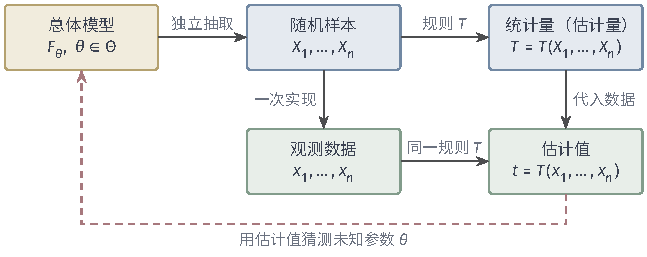
\includegraphics[width=109.6mm]{figures/01-basic-mathematics/05-probability-and-statistics-basics/tikz/est-population-sample-estimate/figure.pdf}
  \caption{总体模型、样本、统计量与估计值的关系。上行（蓝框）是抽样前的随机对象：从总体$F_\theta$独立抽取得到随机样本，再按规则$T$得到统计量（用于估计时称估计量）。下行（绿框）是一次抽样后的数值：观测数据代入同一规则得到估计值。红色虚线表示用估计值去猜测未知参数$\theta$，它是推断而不是计算。}
  \label{fig:est-population-sample-estimate}
\end{figure}

\begin{example}[同一参数的两个估计量]
\label{ex:est-two-estimators}
对测量读数的平均水平$\mu$，样本均值$\frac18\sum_{i=1}^8X_i$是一个估计量，代入读数得估计值$10.1$。“最大读数与最小读数的中点”$\frac12(\max_iX_i+\min_iX_i)$也是一个估计量，代入后得$\frac12(10.4+9.8)=10.1$。两条规则对这组数据恰好给出相同的估计值，但它们是不同的估计量：换一组数据，结果一般就不同了。比较哪条规则更可靠，需要看它们在重复抽样下的表现，这是第~\ref{chap:sampling-errors}章的任务。
\end{example}

\section{经验分布与样本的数值特征}
\label{sec:est-sample-features}

在给出任何模型之前，我们先描述数据本身。第~\ref{chap:random-variables}章用分布函数、期望、方差和分位数描述一个分布；本节把同样的工具用于“把每个观测看成等可能出现”的分布，得到经验分布函数、样本矩、样本方差和样本分位数。

\subsection{经验分布函数}
\label{sec:est-empirical-cdf}

\paragraph{定义与读法}
总体分布函数$F(t)=\mathbb{P}(X\le t)$给出随机变量不超过阈值$t$的概率。手中只有数据时，最自然的替代是数一数有多少个观测不超过$t$，再除以样本量。

\begin{definition}[经验分布函数]
\label{def:est-empirical-cdf}
设$X_1,\dots,X_n$是样本。函数
\begin{equation}
\label{eq:est-empirical-cdf}
\hat F_n(t)=\frac1n\sum_{i=1}^n\mathbb{I}\{X_i\le t\},\qquad t\in\mathbb{R}
\end{equation}
称为\term{经验分布函数}（empirical distribution function），其中$\mathbb{I}\{X_i\le t\}$在$X_i\le t$时取$1$，否则取$0$。在每个观测值上放置概率$1/n$所得的离散分布称为\term{经验分布}（empirical distribution），$\hat F_n$正是它的分布函数。
\end{definition}

$\hat F_n$是一个阶梯函数：它在最小观测值左侧为$0$，在最大观测值处及其右侧为$1$，只在观测值处向上跳跃。若某个值$v$在样本中出现$m$次，则$\hat F_n$在$v$处跳$m/n$；在相邻两个不同观测值之间保持不变。与任何分布函数一样，它右连续，即跳跃点处取跳跃后的值。

\begin{example}[含重复值的读数]
\label{ex:est-ecdf-readings}
将$8$次读数排序为$9.8$、$9.9$、$10.0$、$10.1$、$10.1$、$10.2$、$10.3$、$10.4$，其中$10.1$出现两次。于是
\[
\hat F_8(t)=
\begin{cases}
0, & t<9.8,\\
1/8, & 9.8\le t<9.9,\\
2/8, & 9.9\le t<10.0,\\
3/8, & 10.0\le t<10.1,\\
5/8, & 10.1\le t<10.2,\\
6/8, & 10.2\le t<10.3,\\
7/8, & 10.3\le t<10.4,\\
1, & t\ge10.4 .
\end{cases}
\]
在$10.1$处函数从$3/8$跳到$5/8$，跳跃大小$2/8$等于该值出现的次数除以$8$。例如$\hat F_8(10.15)=5/8$，表示有$62.5\%$的读数不超过$10.15$。
\end{example}

\paragraph{与总体分布函数的区别}
图~\ref{fig:est-empirical-cdf}把这个阶梯与一条假想的总体分布函数画在一起。两者描述的对象不同：总体分布函数$F$是一个确定的函数，描述总体规律；经验分布函数$\hat F_n$只描述当前这$8$个数的累计频率。抽样前，对每个固定的$t$，$\hat F_n(t)$是$n$个取值于$\{0,1\}$的独立随机变量的平均，因此本身是随机变量；换一组数据，阶梯的位置和高度都会改变。图中阶梯大体贴近光滑曲线，但在多处偏离。样本量增大时$\hat F_n(t)$是否会趋于$F(t)$、偏离有多大，属于抽样误差问题，将在第~\ref{sec:samp-lln}节讨论。

\begin{figure}[htbp]
  \centering
  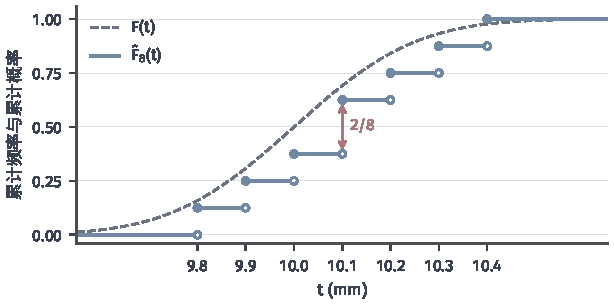
\includegraphics[width=104mm]{figures/01-basic-mathematics/05-probability-and-statistics-basics/matplotlib/est-empirical-cdf/figure.pdf}
  \caption{$8$次读数的经验分布函数（蓝色阶梯）与一条假想的总体分布函数（灰色虚线，取$\mathcal{N}(10.0,0.2^2)$仅作对照）。实心点表示跳跃点处的函数值，空心点表示跳跃前的极限；读数$10.1$出现两次，所以该处跳跃高度为$2/8$，其余各处为$1/8$。}
  \label{fig:est-empirical-cdf}
\end{figure}

\subsection{样本均值与样本矩}

\paragraph{样本均值}
经验分布把概率$1/n$放在每个观测上，按第~\ref{sec:prob-expectation}节的定义，它的期望就是
\begin{equation}
\label{eq:est-sample-mean}
\bar X_n=\frac1n\sum_{i=1}^nX_i ,
\end{equation}
称为\term{样本均值}（sample mean）。不致混淆时省略下标，记作$\bar X$。若数据中有重复值，也可以按不同取值分组：设不同取值为$v_1,\dots,v_m$，各出现$c_1,\dots,c_m$次，则$\bar x=\sum_{j=1}^m v_j\cdot\frac{c_j}{n}$，即“取值乘以频率再求和”，这与离散分布期望的公式完全一致。对读数数据，
\[
\bar x=\frac{9.8+10.1+10.0+10.3+10.1+9.9+10.4+10.2}{8}=\frac{80.8}{8}=10.1 ;
\]
对抽检数据，$\bar x=2/10=0.2$，即不合格品所占比例。

\paragraph{样本原点矩与中心矩}
样本均值只给出数据的位置。第~\ref{chap:random-variables}章用$\mathbb{E}X^k$提取分布的其他数值信息，样本上同样可以对观测的幂取平均。

\begin{definition}[样本矩]
\label{def:est-sample-moments}
设$X_1,\dots,X_n$是样本，$k$为正整数。称
\[
m_k=\frac1n\sum_{i=1}^nX_i^k
\qquad\text{与}\qquad
\hat\mu_k=\frac1n\sum_{i=1}^n(X_i-\bar X)^k
\]
分别为$k$阶\term{样本原点矩}（sample raw moment）和$k$阶\term{样本中心矩}（sample central moment），统称\term{样本矩}（sample moment）。
\end{definition}

原点矩以$0$为参照，中心矩以样本均值为参照。一阶原点矩就是样本均值；一阶中心矩恒为$0$，因为$\sum_i(X_i-\bar X)=0$；二阶中心矩度量观测围绕均值的分散程度。两者可以互相换算，例如展开平方得
\begin{equation}
\label{eq:est-second-moment-identity}
\hat\mu_2=\frac1n\sum_{i=1}^n(X_i^2-2\bar XX_i+\bar X^2)=m_2-2\bar X\cdot\bar X+\bar X^2=m_2-\bar X^2 .
\end{equation}

\begin{example}[读数的样本矩]
\label{ex:est-reading-moments}
读数与均值$10.1$的离差为$-0.3$、$0$、$-0.1$、$0.2$、$0$、$-0.2$、$0.3$、$0.1$，平方和为$0.28$，所以$\hat\mu_2=0.28/8=0.035$。另一方面，$m_2=\frac18\sum_ix_i^2=102.045$，按式~\eqref{eq:est-second-moment-identity}有$m_2-\bar x^2=102.045-102.01=0.035$，两种算法一致。离差关于$0$正负对称，所以三阶中心矩$\hat\mu_3=0$；四阶中心矩$\hat\mu_4=(2\times0.3^4+2\times0.2^4+2\times0.1^4)/8=0.00245$。
\end{example}

\paragraph{能算出不等于总体矩存在}
任意有限个实数都能算出任意阶样本矩，但这并不说明对应的总体矩存在。例如标准Cauchy分布的密度为$f(x)=\frac{1}{\pi(1+x^2)}$，由于$\int_0^\infty\frac{x}{\pi(1+x^2)}\,\mathrm{d}x=\lim_{b\to\infty}\frac{\ln(1+b^2)}{2\pi}=\infty$，它的期望不存在。从这个分布抽出的样本仍然有样本均值，只是这个数并不对应任何总体均值。用样本矩去推断总体矩之前，必须先确认后者存在。

\subsection{样本方差}
\label{sec:est-sample-variance}

\paragraph{两种分母}
描述数据的分散程度，最直接的是平方离差的平均$\hat\sigma_n^2=\frac1n\sum_i(X_i-\bar X)^2$，也就是二阶样本中心矩$\hat\mu_2$。实际中更常用的是把分母换成$n-1$的版本。

\begin{definition}[样本方差]
\label{def:est-sample-variance}
设$n\ge2$。称
\begin{equation}
\label{eq:est-sample-variance}
S_n^2=\frac{1}{n-1}\sum_{i=1}^n(X_i-\bar X_n)^2
\end{equation}
为\term{修正样本方差}（corrected sample variance），通常简称\term{样本方差}（sample variance）；称$S_n=\sqrt{S_n^2}$为\term{样本标准差}（sample standard deviation）。分母为$n$的$\hat\sigma_n^2=\frac{n-1}{n}S_n^2$称为未修正的样本方差。
\end{definition}

对读数数据，平方离差和为$0.28$，所以$\hat\sigma^2=0.28/8=0.035$，$S^2=0.28/7=0.04$，$S=0.2$。两者相差一个因子$8/7$。样本量越大，这个因子越接近$1$；样本量很小时，差别不能忽略。为什么要除以$n-1$，可以从期望的计算中看出来。

\paragraph{期望的计算}
下面的定理在独立同分布、总体方差有限的条件下计算平方离差和的期望。证明需要两个事实：期望是线性的；相互独立的随机变量之和的方差等于各方差之和（第~\ref{sec:rvec-moments}节），从而$\operatorname{Var}(\bar X_n)=\frac{1}{n^2}\sum_i\operatorname{Var}(X_i)=\sigma^2/n$。

\begin{theorem}[平方离差和的期望]
\label{thm:est-sample-variance-expectation}
设$n\ge2$，$X_1,\dots,X_n$独立同分布，$\mathbb{E}X_1=\mu$，$\operatorname{Var}(X_1)=\sigma^2<\infty$。则
\[
\mathbb{E}\Big[\sum_{i=1}^n(X_i-\bar X_n)^2\Big]=(n-1)\sigma^2,
\qquad\text{从而}\qquad
\mathbb{E}S_n^2=\sigma^2,\quad \mathbb{E}\hat\sigma_n^2=\frac{n-1}{n}\sigma^2 .
\]
\end{theorem}

\begin{proof}
先把围绕真实均值$\mu$的平方和分解为两部分。将$X_i-\mu$写成$(X_i-\bar X_n)+(\bar X_n-\mu)$，展开平方并求和：
\[
\sum_{i=1}^n(X_i-\mu)^2=\sum_{i=1}^n(X_i-\bar X_n)^2+2(\bar X_n-\mu)\sum_{i=1}^n(X_i-\bar X_n)+n(\bar X_n-\mu)^2 .
\]
中间一项含因子$\sum_i(X_i-\bar X_n)=0$，因此
\begin{equation}
\label{eq:est-sum-of-squares-decomposition}
\sum_{i=1}^n(X_i-\bar X_n)^2=\sum_{i=1}^n(X_i-\mu)^2-n(\bar X_n-\mu)^2 .
\end{equation}
对右边逐项取期望。每个$X_i$的方差为$\sigma^2$，所以$\mathbb{E}\sum_i(X_i-\mu)^2=n\sigma^2$。又因$\mathbb{E}\bar X_n=\mu$，有$\mathbb{E}(\bar X_n-\mu)^2=\operatorname{Var}(\bar X_n)=\sigma^2/n$，故$\mathbb{E}\,n(\bar X_n-\mu)^2=\sigma^2$。两者相减得$(n-1)\sigma^2$。分别除以$n-1$和$n$即得后两个等式。
\end{proof}

式~\eqref{eq:est-sum-of-squares-decomposition}说明了修正因子的来源。围绕真实均值$\mu$的平方和平均为$n\sigma^2$，但$\mu$未知，我们只能围绕$\bar X_n$计算。$\bar X_n$是由同一组数据算出的，它总是落在数据“中间”，使平方和比围绕$\mu$时更小，平均少了一个$\sigma^2$。除以$n-1$恰好补偿了这部分损失。注意定理需要$n\ge2$：只有一个观测时，离差恒为$0$，无法从数据中看出分散程度。

一个估计量的期望是否等于被估计的量，只是评价估计的一个角度；除以$n-1$的估计并不在所有意义下都更好。估计的系统误差、波动和均方误差怎样定义和比较，留到第~\ref{sec:samp-errors}节统一讨论。

\begin{example}[两个观测的平方离差]
\label{ex:est-two-observations}
取$n=2$。此时$\bar X=\frac{X_1+X_2}2$，$\sum_i(X_i-\bar X)^2=\frac{(X_1-X_2)^2}{2}$。由于$X_1-X_2$的均值为$0$，方差为$2\sigma^2$，有$\mathbb{E}(X_1-X_2)^2=2\sigma^2$，所以平方离差和的期望为$\sigma^2=(2-1)\sigma^2$，与定理一致。若误用分母$n=2$，得到的$\hat\sigma^2$平均只有$\sigma^2/2$。
\end{example}

\subsection{样本分位数}

\paragraph{顺序统计量}
分位数描述分布的位置而不是平均，它需要把数据排序。

\begin{definition}[顺序统计量]
\label{def:est-order-statistics}
把样本$X_1,\dots,X_n$从小到大排列为$X_{(1)}\le X_{(2)}\le\dots\le X_{(n)}$，称$X_{(k)}$为第$k$个\term{顺序统计量}（order statistic）。
\end{definition}

$X_{(1)}=\min_iX_i$与$X_{(n)}=\max_iX_i$分别是样本最小值和最大值，二者之差$X_{(n)}-X_{(1)}$称为极差。位于中间位置的顺序统计量给出数据的“中心”：它左右两侧的观测个数大致相等，与样本均值不同，它不受个别极端值的大小影响。对读数数据，$x_{(1)}=9.8$，$x_{(8)}=10.4$，$x_{(4)}=x_{(5)}=10.1$。

\paragraph{由经验分布函数定义分位数}
第~\ref{sec:prob-numerical-features}节用分布函数的广义逆定义总体分位数：$p$分位数是使$F(t)\ge p$的最小$t$。对经验分布函数做同样的操作，就得到样本分位数。

\begin{definition}[样本分位数]
\label{def:est-sample-quantile}
设$0<p<1$。称
\begin{equation}
\label{eq:est-sample-quantile}
\hat q_p=\min\{t\in\mathbb{R}:\hat F_n(t)\ge p\}=X_{(\lceil np\rceil)}
\end{equation}
为$p$\term{样本分位数}（sample quantile），其中$\lceil np\rceil$是不小于$np$的最小整数。$p=1/2$时的样本分位数称为\term{样本中位数}（sample median）。
\end{definition}

第二个等号可以这样验证。$\hat F_n$在$X_{(k)}$处的值至少是$k/n$，而在$X_{(k)}$左侧的值至多是$(k-1)/n$。因此使$\hat F_n(t)\ge p$的最小$t$，就是满足$k/n\ge p$的最小$k$所对应的$X_{(k)}$，即$k=\lceil np\rceil$。

\paragraph{不同的约定}
当$np$恰为整数时，$\hat F_n$在$X_{(np)}$与$X_{(np+1)}$之间恰好等于$p$，整段区间上的点都“处于$p$的位置”，取左端点只是一种选择。常见的约定有以下几种。
\begin{itemize}
  \item 广义逆：按式~\eqref{eq:est-sample-quantile}取$X_{(\lceil np\rceil)}$。
  \item 跳跃处取中点：$np$为整数时取$\frac12(X_{(np)}+X_{(np+1)})$，否则同上。偶数样本的中位数$\frac12(X_{(n/2)}+X_{(n/2+1)})$就是这种约定在$p=1/2$时的结果。
  \item 线性插值：令$h=(n-1)p+1$，取$X_{(\lfloor h\rfloor)}+(h-\lfloor h\rfloor)\big(X_{(\lfloor h\rfloor+1)}-X_{(\lfloor h\rfloor)}\big)$，即把第$k$个顺序统计量放在$p=(k-1)/(n-1)$处，相邻两点之间用直线连接。
\end{itemize}
图~\ref{fig:est-sample-quantiles}把广义逆与线性插值两种约定看成$p$的函数画了出来：广义逆是经验分布函数阶梯的“反函数”，也呈阶梯形，在$p$越过每个$k/n$时跳到下一个顺序统计量；线性插值则是一条穿过各顺序统计量的折线。

\begin{example}[读数的四分位数与中位数]
\label{ex:est-quantile-conventions}
对$8$个读数取$p=0.25$，$np=2$是整数。广义逆给出$x_{(2)}=9.9$；跳跃处取中点给出$\frac12(9.9+10.0)=9.95$；线性插值中$h=7\times0.25+1=2.75$，给出$9.9+0.75\times(10.0-9.9)=9.975$。三种约定得到三个不同的值。

对中位数，三种约定都给出$10.1$，因为两个中间值$x_{(4)}=x_{(5)}=10.1$相同。若只取前$6$个读数，排序后为$9.8,9.9,10.0,10.1,10.1,10.3$，中间两个值是$10.0$与$10.1$：广义逆给出$x_{(3)}=10.0$，后两种约定都给出$10.05$。
\end{example}

\begin{figure}[htbp]
  \centering
  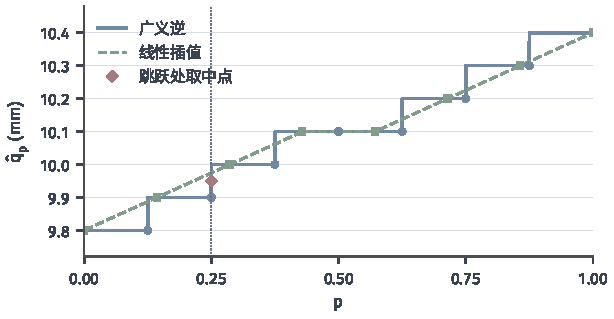
\includegraphics[width=104mm]{figures/01-basic-mathematics/05-probability-and-statistics-basics/matplotlib/est-sample-quantiles/figure.pdf}
  \caption{$8$个读数的样本分位数$\hat q_p$随$p$的变化。蓝色阶梯是经验分布函数的广义逆，圆点标出它在$p=k/8$处取到的顺序统计量$x_{(k)}$；绿色虚线是线性插值约定，方点位于$p=(k-1)/7$。在$p=0.25$（点线）处，广义逆取$9.9$，跳跃处取中点得$9.95$（菱形），线性插值得$9.975$。}
  \label{fig:est-sample-quantiles}
\end{figure}

不同统计软件默认采用的约定并不相同，样本量较小时，同一组数据可能报告出不同的分位数。这些差别局限在$p$所在位置附近的少数几个顺序统计量之间，样本量增大、数据变密时一般会缩小。报告分位数时，应当说明所用的约定。

\section{矩估计}
\label{sec:est-moments}

上一节的样本矩只描述数据。如果再给出统计模型，总体矩就成了参数的函数；让总体矩等于样本矩，便得到关于参数的方程。这是构造估计最直接的方法。

\subsection{矩估计的构造}

\paragraph{估计方程}
在统计模型$\{F_\theta:\theta\in\Theta\}$下，设$X\sim F_\theta$的$k$阶矩存在，把它记作
\[
\mu_k(\theta)=\mathbb{E}_\theta X^k ,
\]
下标$\theta$提示期望是在分布$F_\theta$下计算的。$\mu_k(\theta)$是参数的一个已知函数，而样本原点矩$m_k$可以由数据算出。若参数有$d$个分量，我们选取$d$个矩，令它们分别等于对应的样本矩：
\begin{equation}
\label{eq:est-moment-equations}
\mu_k(\theta)=m_k,\qquad k=1,\dots,d .
\end{equation}

\begin{definition}[矩估计]
\label{def:est-method-of-moments}
若方程组~\eqref{eq:est-moment-equations}在$\Theta$中有唯一解，则称这个解$\hat\theta_n$为$\theta$的\term{矩估计}（method of moments estimator）。
\end{definition}

这一做法的依据是第~\ref{sec:est-sample-features}节的观察：样本矩是经验分布的矩，而经验分布描述了数据的累计频率。若经验分布接近总体分布，它们的矩也应当接近，于是解出的参数应当接近真实参数。这种“接近”在什么条件下成立，第~\ref{sec:samp-consistency}节再作说明。

\paragraph{计算步骤}
矩估计的计算可以按四步组织：
\begin{enumerate}
  \item 选择矩：确定使用哪几阶矩，也可以使用中心矩或其他函数的期望；
  \item 建立方程：把所选总体矩写成参数的函数，令其等于对应样本矩；
  \item 求解参数：解方程组，得到用样本矩表示的参数；
  \item 检查范围：确认解存在、唯一，并落在参数集$\Theta$中。
\end{enumerate}
第一步中，方程个数等于参数个数只是一个计数条件，并不保证方程组相互独立或可解。例如对只取$0$和$1$的随机变量，总有$X^k=X$，所以各阶原点矩全部等于$\mathbb{E}X$：无论选择几阶原点矩，得到的都是同一个方程。若模型有两个参数，而数据只取$0$和$1$，原点矩就不足以确定参数。第四步的检查同样不能省略，本节最后一小节将给出解不存在、不唯一或与数据矛盾的例子。

\subsection{矩估计的计算}

\paragraph{单参数模型}
单参数模型只需一个方程，通常选一阶矩。

\begin{example}[Bernoulli与Poisson模型]
\label{ex:est-mom-bernoulli-poisson}
在Bernoulli模型下，$\mu_1(p)=\mathbb{E}_pX=p$，方程$p=m_1$直接给出$\hat p=\bar X$。对抽检数据，$\hat p=2/10=0.2$，即不合格率的矩估计就是样本中不合格品的比例。这个解总在$[0,1]$中，第四步自动满足。

在Poisson模型下，$\mathbb{E}_\lambda X=\lambda$，所以同样有$\hat\lambda=\bar X$。若某客服中心连续$8$天收到的投诉次数为$2,0,3,1,2,4,1,3$（教学示例），则$\hat\lambda=16/8=2$，即估计每天平均收到$2$次投诉。若$8$天都没有投诉，$\hat\lambda=0$不在参数集$(0,\infty)$中，此时矩估计不存在；这种边界情况在第~\ref{sec:est-mle}节还会遇到。
\end{example}

两个模型中样本均值都成为参数的估计，原因是参数恰好等于总体均值。若参数与均值的关系不是恒等的，就需要解方程。例如指数分布$f(x;\lambda)=\lambda e^{-\lambda x}$的均值为$1/\lambda$，方程$1/\lambda=\bar X$给出$\hat\lambda=1/\bar X$。

\paragraph{两参数高斯模型}
均值和方差都未知时，需要两个方程。高斯分布$\mathcal{N}(\mu,\sigma^2)$的前两阶原点矩为$\mu_1=\mu$，$\mu_2=\mathbb{E}X^2=\operatorname{Var}(X)+(\mathbb{E}X)^2=\sigma^2+\mu^2$。令它们等于样本矩：
\[
\mu=m_1,\qquad \sigma^2+\mu^2=m_2 .
\]
第一式给出$\hat\mu=\bar X$，代入第二式并利用式~\eqref{eq:est-second-moment-identity}，得
\begin{equation}
\label{eq:est-mom-gaussian}
\hat\mu=\bar X,\qquad \hat\sigma^2=m_2-\bar X^2=\frac1n\sum_{i=1}^n(X_i-\bar X)^2 .
\end{equation}
方差的矩估计正是分母为$n$的未修正样本方差。

\begin{example}[读数的矩估计]
\label{ex:est-mom-readings}
由例~\ref{ex:est-reading-moments}，$m_1=10.1$，$m_2=102.045$。按式~\eqref{eq:est-mom-gaussian}，$\hat\mu=10.1$，$\hat\sigma^2=102.045-10.1^2=0.035$，$\hat\sigma\approx0.187$。修正样本方差为$S^2=0.04$，比矩估计大$8/7$倍。
\end{example}

这里的分母为$n$不是计算失误，而是矩估计的直接结果：矩估计让模型方差等于经验分布的方差，而经验分布的方差的分母就是$n$。定理~\ref{thm:est-sample-variance-expectation}表明，这个估计的期望是$\frac{n-1}{n}\sigma^2$，略小于$\sigma^2$。两种分母各自的含义已经清楚，但哪一个“更好”需要先确定评价标准，留给第~\ref{sec:samp-errors}节。

\subsection{解的存在性与适用条件}

\paragraph{需要检查的三件事}
矩估计的方程容易写出，但不能直接认为它给出了合理的估计。使用前至少要检查三点：所选的总体矩是否存在，否则方程本身没有意义（如前述Cauchy分布）；所选的矩能否确定待估参数，即不同参数是否对应不同的矩；解是否存在、唯一，并且与参数集及数据相容。下面两个例子分别对应后两点。

\begin{example}[解与数据矛盾]
\label{ex:est-mom-uniform}
设$X\sim\operatorname{U}(0,\theta)$，$\theta>0$未知。由$\mathbb{E}_\theta X=\theta/2$得矩估计$\hat\theta=2\bar X$。若观测为$0.2,\ 0.3,\ 1.9$，则$\bar x=0.8$，$\hat\theta=1.6$。但数据中已经有观测$1.9>1.6$，而在$\operatorname{U}(0,1.6)$下不可能出现大于$1.6$的值。这个估计值虽然在参数集$(0,\infty)$中，却与数据本身矛盾。矩方程只用到数据的平均，没有用到“所有观测都不超过$\theta$”这一信息。
\end{example}

\begin{example}[只用二阶矩丢失符号]
\label{ex:est-mom-sign}
设$X\sim\mathcal{N}(\mu,1)$。若只用二阶矩，方程为$\mu^2+1=m_2$。对观测$-1.2,\ -0.8,\ -1.5,\ -0.5$，$m_2=(1.44+0.64+2.25+0.25)/4=1.145$，解得$\mu=\pm\sqrt{0.145}\approx\pm0.381$，两个解无法区分；而样本均值为$-1.0$，明确指向负值。原因在于$\mathbb{E}X^2$只取决于$\mu^2$，参数$\mu$与$-\mu$给出相同的二阶矩，二阶矩不能确定$\mu$的符号。更糟的是，若观测为$0.3,\ -0.2,\ 0.5$，$m_2\approx0.127<1$，方程无实数解。改用一阶矩$\mu=m_1$，两个问题都不出现。
\end{example}

\paragraph{高阶矩对极端观测敏感}
需要多个方程时，自然会想到使用三阶、四阶矩，但高阶矩有一个实际缺陷：它们对个别极端观测非常敏感。离差先取高次幂再平均，一个大的离差会被放大到压倒其他所有项。

\begin{example}[一个读数的错误]
\label{ex:est-moment-sensitivity}
若把读数中的$10.4$误记为$11.4$，样本均值从$10.1$变为$10.225$，只改变约$1\%$；二阶中心矩从$0.035$变为约$0.219$，增大到约$6$倍；四阶中心矩从$0.00245$变为约$0.244$，增大到约$100$倍。基于高阶矩的估计因此可能被一个异常值左右。
\end{example}

因此，矩估计适合于参数可以由低阶矩直接确定的模型。它计算简单，常用来得到初步估计，或者为后面需要迭代求解的方法提供初值。

\section{最大似然估计}
\label{sec:est-mle}

矩估计只使用数据的几个平均量。例~\ref{ex:est-mom-uniform}显示，这可能丢掉数据中的其他信息。另一种思路是直接利用模型给出的整个联合分布：在所有候选参数中，选择使当前数据出现的概率（或密度）最大的那一个。

\subsection{似然函数}

\paragraph{固定数据，变动参数}
式~\eqref{eq:est-sample-joint}给出的联合质量函数$p(x_1,\dots,x_n;\theta)$有两个自变量：数据和参数。计算概率时，我们固定$\theta$，看不同数据出现的可能性。估计时情形反过来：数据已经观察到，是固定的；未知的是$\theta$。于是我们把同一个表达式看作$\theta$的函数，比较不同参数下“观察到这组数据”的可能性大小。

\begin{definition}[似然函数]
\label{def:est-likelihood}
给定观测值$x_1,\dots,x_n$，称
\[
L(\theta)=L(\theta;x_1,\dots,x_n)=p(x_1,\dots,x_n;\theta)\quad\text{（离散情形）}
\]
或$L(\theta)=f(x_1,\dots,x_n;\theta)$（连续情形）为参数$\theta$的\term{似然函数}（likelihood function），$\theta\in\Theta$。若$L(\theta)>0$，称$\ell(\theta)=\ln L(\theta)$为\term{对数似然函数}（log-likelihood function）。
\end{definition}

对随机样本，由式~\eqref{eq:est-sample-joint}，似然是各观测概率或密度的乘积，对数似然是相应的和：
\begin{equation}
\label{eq:est-log-likelihood}
L(\theta)=\prod_{i=1}^n f(x_i;\theta),\qquad
\ell(\theta)=\sum_{i=1}^n\ln f(x_i;\theta) .
\end{equation}
因为对数函数严格递增，$L$与$\ell$在同样的参数处取最大值；而和比积更容易求导，所以计算时几乎总是使用对数似然。数值上，许多小于$1$的数连乘会迅速接近$0$，取对数也避免了这个问题。

\paragraph{似然不是参数的分布}
似然函数比较的是同一组数据在不同参数下的概率，它本身不是参数的概率分布。$L(\theta_1)>L(\theta_2)$表示“若参数为$\theta_1$，看到这组数据的可能性更大”，而不是“$\theta_1$为真的概率更大”。

\begin{example}[似然的积分不为一]
\label{ex:est-likelihood-not-density}
例~\ref{ex:est-joint-bernoulli}给出抽检数据的似然$L(p)=p^2(1-p)^8$，$p\in[0,1]$。把它看作$p$的函数在$[0,1]$上积分，利用Beta函数（第~\ref{sec:prob-beta}节）$\int_0^1p^{a-1}(1-p)^{b-1}\mathrm{d}p=\frac{(a-1)!\,(b-1)!}{(a+b-1)!}$（$a,b$为正整数），得
\[
\int_0^1p^2(1-p)^8\,\mathrm{d}p=\frac{2!\,8!}{11!}=\frac{1}{495}\neq1 .
\]
所以$L(p)$不是$p$的密度。似然只有比值有意义：把$L$乘以任何不依赖$\theta$的正常数，最大值的位置不变。
\end{example}

\subsection{最大似然估计的计算}

似然函数给出了比较参数的依据，自然的做法是在参数集中选出似然最大的参数。

\begin{definition}[最大似然估计]
\label{def:est-mle}
若存在$\hat\theta\in\Theta$，使得对所有$\theta\in\Theta$都有$L(\hat\theta)\ge L(\theta)$，则称$\hat\theta$为$\theta$的\term{最大似然估计}（maximum likelihood estimate，MLE）。把$\hat\theta$看作数据的函数时，得到最大似然估计量。
\end{definition}

计算通常分三步：写出对数似然；在参数集内部令导数为零，求出候选解；检查候选解确实是最大值点，并与边界及趋于无穷时的情形作比较。第三步不能省略，本节最后一小节会说明原因。

\paragraph{Bernoulli模型}
先看抽检数据。Bernoulli模型只有一个参数，对数似然是一元函数，可以直接用一元微分求最大值。

\begin{example}[不合格率的最大似然估计]
\label{ex:est-mle-bernoulli}
设$X_1,\dots,X_n\overset{\text{i.i.d.}}{\sim}\operatorname{Bernoulli}(p)$，记不合格件数$k=\sum_ix_i$。似然为$L(p)=p^k(1-p)^{n-k}$。设$0<k<n$，对$p\in(0,1)$，
\[
\ell(p)=k\ln p+(n-k)\ln(1-p),\qquad
\ell'(p)=\frac{k}{p}-\frac{n-k}{1-p}.
\]
令$\ell'(p)=0$，得$k(1-p)=(n-k)p$，即$p=k/n$。又$\ell''(p)=-\frac{k}{p^2}-\frac{n-k}{(1-p)^2}<0$，$\ell$在$(0,1)$上严格凹（第~\ref{chap:univariate-differentiation}章），所以$k/n$是$(0,1)$上唯一的最大值点；而在两个端点处$L(0)=L(1)=0$，比内部的值都小。因此$\hat p=k/n=\bar x$。对抽检数据，$\hat p=2/10=0.2$，与矩估计相同。
\end{example}

图~\ref{fig:est-bernoulli-loglik}的左图画出了$n=10$、$k=2$时的对数似然：曲线在$p=0.2$处取最大值，向两侧下降，靠近$p=0$和$p=1$时趋于$-\infty$。右图对应下一小节将讨论的边界情形。

\begin{figure}[htbp]
  \centering
  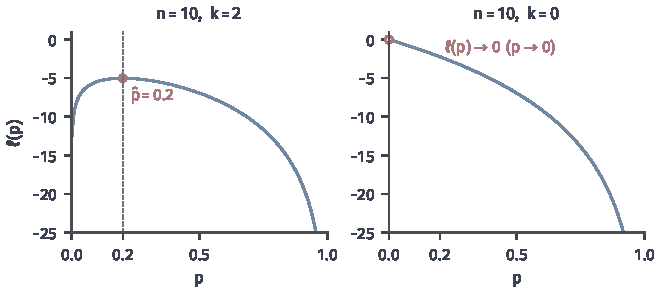
\includegraphics[width=112mm]{figures/01-basic-mathematics/05-probability-and-statistics-basics/matplotlib/est-bernoulli-loglik/figure.pdf}
  \caption{$10$次Bernoulli观测的对数似然$\ell(p)=k\ln p+(10-k)\ln(1-p)$。左：抽检数据$k=2$，曲线在$\hat p=0.2$处取得内部最大值。右：$10$件全部合格（$k=0$），$\ell(p)=10\ln(1-p)$在$(0,1)$上严格递减，上确界$0$只在端点$p=0$处达到（空心圆）。纵轴在$-25$处截断。}
  \label{fig:est-bernoulli-loglik}
\end{figure}

\paragraph{高斯均值模型}
再看读数数据，先假定测量方差已知，只估计均值。这时对数似然中依赖参数的部分是一个平方和，用配方比求导更直接。

\begin{example}[已知方差时高斯均值的最大似然估计]
\label{ex:est-mle-gaussian-mean}
设$X_i\sim\mathcal{N}(\mu,\sigma^2)$，$\sigma^2$已知，只估计$\mu$。由高斯密度$f(x;\mu)=\frac{1}{\sqrt{2\pi}\sigma}\exp\!\big(-\frac{(x-\mu)^2}{2\sigma^2}\big)$，
\[
\ell(\mu)=-\frac n2\ln(2\pi\sigma^2)-\frac{1}{2\sigma^2}\sum_{i=1}^n(x_i-\mu)^2 .
\]
第一项与$\mu$无关，所以最大化$\ell$等价于最小化平方和$\sum_i(x_i-\mu)^2$。利用与式~\eqref{eq:est-sum-of-squares-decomposition}相同的分解，$\sum_i(x_i-\mu)^2=\sum_i(x_i-\bar x)^2+n(\bar x-\mu)^2$，第二项在$\mu=\bar x$时为零、其余时候为正，因此$\hat\mu=\bar x$，无需求导。对读数数据，$\hat\mu=10.1$。高斯误差下的最大似然因而化为最小二乘，这一联系在第~\ref{chap:linear-equations-and-optimization}章的最小二乘问题中还会以向量形式出现。
\end{example}

\paragraph{均值与方差都未知}
现在把均值和方差同时作为参数。为了求导方便，把方差记作$v=\sigma^2>0$。记$\mathrm{SS}(\mu)=\sum_i(x_i-\mu)^2$，对数似然为
\[
\ell(\mu,v)=-\frac n2\ln(2\pi)-\frac n2\ln v-\frac{\mathrm{SS}(\mu)}{2v},\qquad \mu\in\mathbb{R},\ v>0 .
\]
我们分两步求最大值。第一步，固定任意$v>0$，$\ell$作为$\mu$的函数在$\mu=\bar x$处最大，理由同上例。所以对每个$v$都有$\ell(\mu,v)\le\ell(\bar x,v)$。第二步，记$\mathrm{SS}=\mathrm{SS}(\bar x)=\sum_i(x_i-\bar x)^2$，并假定$\mathrm{SS}>0$，即观测不全相同。考虑一元函数
\[
g(v)=\ell(\bar x,v)=-\frac n2\ln(2\pi)-\frac n2\ln v-\frac{\mathrm{SS}}{2v},\qquad
g'(v)=-\frac{n}{2v}+\frac{\mathrm{SS}}{2v^2}=\frac{\mathrm{SS}-nv}{2v^2}.
\]
$g'(v)$在$v<\mathrm{SS}/n$时为正，在$v>\mathrm{SS}/n$时为负，所以$g$在$v=\mathrm{SS}/n$处取最大值。合并两步，最大似然估计为
\begin{equation}
\label{eq:est-mle-gaussian}
\hat\mu=\bar x,\qquad
\hat\sigma^2=\frac1n\sum_{i=1}^n(x_i-\bar x)^2 .
\end{equation}

\begin{example}[读数的最大似然估计]
\label{ex:est-mle-readings}
对读数数据，$\hat\mu=10.1$，$\hat\sigma^2=0.28/8=0.035$，$\hat\sigma\approx0.187$。图~\ref{fig:est-gaussian-contours}画出对数似然在$(\mu,\sigma)$平面上的等高线：等高线围绕最大值点呈封闭的卵形，在$\sigma$方向上不对称，下方（$\sigma$较小）排列更密，说明把$\sigma$估小比估大使似然下降得更快。
\end{example}

\begin{figure}[htbp]
  \centering
  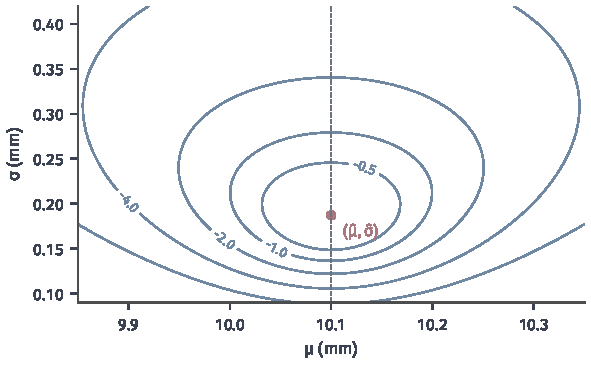
\includegraphics[width=100mm]{figures/01-basic-mathematics/05-probability-and-statistics-basics/matplotlib/est-gaussian-contours/figure.pdf}
  \caption{$8$个读数在高斯模型下的对数似然等高线，以$(\mu,\sigma)$为坐标。各等高线标注的是与最大值之差，由内向外依次为$-0.5,-1,-2,-4,-8$（最外一条未标注）。红点为最大似然估计$(\hat\mu,\hat\sigma)=(10.1,0.187)$，虚线$\mu=\bar x$上各点是固定$\sigma$时对$\mu$的最优选择。}
  \label{fig:est-gaussian-contours}
\end{figure}

把式~\eqref{eq:est-mle-gaussian}与前面的结果放在一起比较：方差的最大似然估计与矩估计~\eqref{eq:est-mom-gaussian}相同，分母都是$n$，而修正样本方差的分母是$n-1$。最大似然估计的分母为$n$，是因为它要使当前数据的似然最大；在$\mu$取$\bar x$之后，对数似然对$v$的最优点恰好是平方离差的平均。它并不以“期望等于$\sigma^2$”为目标，所以与定理~\ref{thm:est-sample-variance-expectation}给出的修正因子无关。两种分母代表两种不同的构造原则，而不是一对一错。

\subsection{边界解与解的存在性}

上面的例子中，最大值都在参数集内部取得，令导数为零就找到了它。本小节说明，这一做法可能失效：最大值可能落在边界上，也可能根本不存在。

\paragraph{边界上的最大值}
Bernoulli的推导假定了$0<k<n$。若抽检中一件不合格品都没有出现，导数就不再有零点。

\begin{example}[全部合格]
\label{ex:est-mle-boundary}
若抽检的$10$件产品全部合格，即$k=0$，则$L(p)=(1-p)^{10}$，$\ell(p)=10\ln(1-p)$。对$p\in(0,1)$，$\ell'(p)=-\frac{10}{1-p}<0$，导数在内部没有零点，对数似然严格递减（图~\ref{fig:est-bernoulli-loglik}右）。

结论取决于参数集。若$\Theta=[0,1]$，$L$在端点$p=0$处取得最大值$L(0)=1$，最大似然估计为$\hat p=0$。若出于“不合格率不可能恰为$0$”的考虑把参数集取为$(0,1)$，则对每个$p\in(0,1)$，都有更小的$p'$使$L(p')>L(p)$；$\sup_{0<p<1}L(p)=1$，但没有任何参数达到它，最大似然估计不存在。同样的讨论适用于全部不合格的情形$k=n$。
\end{example}

全部合格时给出$\hat p=0$，意味着“认为这条生产线永远不会出次品”，只凭$10$件产品显然不足以下这样的结论。这个问题来自数据太少，而不是计算错误；第~\ref{sec:est-bayes}节的后验估计会给出一种在内部取值的替代。

\paragraph{似然无界}
高斯模型的推导在第二步假定了$\mathrm{SS}>0$。如果所有观测都相同，情况完全不同。

\begin{example}[全部观测相同]
\label{ex:est-mle-unbounded}
设$3$次读数都是$10.0$。取$\mu=10.0$，则$\mathrm{SS}(\mu)=0$，对数似然化为
\[
\ell(10.0,\sigma)=-3\ln\sigma-\frac32\ln(2\pi).
\]
当$\sigma\to0^+$时，它趋于$+\infty$。似然在$\mu\in\mathbb{R}$、$\sigma>0$上没有上界，因此不存在最大似然估计。形式上代入式~\eqref{eq:est-mle-gaussian}会得到$\hat\sigma^2=0$，但它不在参数集$(0,\infty)$中，不是任何高斯分布的方差。
\end{example}

图~\ref{fig:est-unbounded-likelihood}把这一情形与读数互不相同的样本对照。观测略有差异时，$\mathrm{SS}>0$使$-\mathrm{SS}/(2\sigma^2)$在$\sigma\to0$时趋于$-\infty$，压过了$-n\ln\sigma$的增长，曲线在内部出现最大值；观测完全相同时，前一项消失，只剩下无限增长的$-n\ln\sigma$。对连续模型，样本中出现完全相同的值往往是仪器分辨率有限、数据被取整的结果，此时应当重新考虑模型是否恰当。

\begin{figure}[htbp]
  \centering
  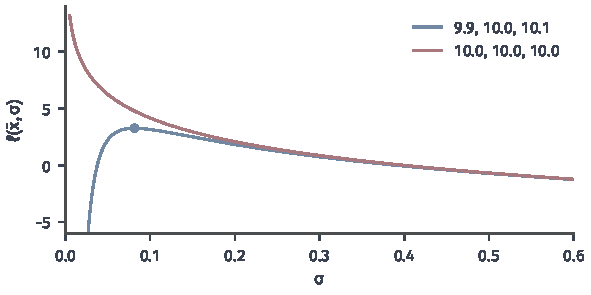
\includegraphics[width=100mm]{figures/01-basic-mathematics/05-probability-and-statistics-basics/matplotlib/est-unbounded-likelihood/figure.pdf}
  \caption{取$\mu=\bar x$时高斯对数似然随$\sigma$的变化。蓝线：读数$9.9,10.0,10.1$，曲线在$\hat\sigma=\sqrt{0.02/3}\approx0.082$处取得最大值（圆点）。红线：三个读数都等于$10.0$，平方离差和为零，对数似然$-3\ln\sigma-\frac32\ln(2\pi)$在$\sigma\to0$时无限增大，最大值不存在。纵轴在$14$处截断。}
  \label{fig:est-unbounded-likelihood}
\end{figure}

\paragraph{最大值、上确界与无界}
两个例子提示我们区分三种情形：似然在参数集中取得最大值，最大似然估计存在；似然有上确界但不被任何参数取到，如参数集为$(0,1)$时的全部合格数据；似然无上界，如全部观测相同的高斯数据。令导数为零只能找出参数集内部的候选点，不能区分这三种情形。完整的计算必须检查参数集的边界，以及参数趋于边界或无穷远时似然的走向。

\section{基于先验与后验的估计}
\label{sec:est-bayes}

矩估计和最大似然估计都只使用当前数据。实际问题中，我们在看到数据之前往往已经对参数有所了解：同类生产线的不合格率通常在$10\%$左右，或者仪器的标称长度是$10.0$mm。本节用概率分布表示这种了解，再用Bayes公式把它与数据合并，最后从合并后的分布中提取估计。

\subsection{先验分布}

\paragraph{参数的不确定性}
前几节把参数看作未知的常数。现在我们换一个角度：既然不知道$\theta$，就用一个概率分布描述“$\theta$可能在哪里，各处的可能性有多大”。这个分布描述的是我们对参数的认识程度，而不是参数自身在随机变化。

\begin{definition}[先验分布]
\label{def:est-prior}
在统计模型$\{F_\theta:\theta\in\Theta\}$中，把参数看作取值于$\Theta$的随机变量，并给定它的分布$\pi(\theta)$（质量函数或密度），称为\term{先验分布}（prior distribution）。观测模型$p(x\mid\theta)$或$f(x\mid\theta)$表示给定参数后数据的条件分布。先验分布中用于调节位置和形状的常数称为\term{超参数}（hyperparameter）。
\end{definition}

于是有两层分布：先验$\pi(\theta)$描述参数的不确定性；观测模型描述参数给定后，个体观测的随机性。这正对应第~\ref{sec:est-samples}节区分的两种不确定性。先验的取值范围必须与参数集一致，例如不合格率的先验只能放在$[0,1]$上；在独立同分布模型中，给定$\theta$后各观测条件独立，联合条件密度仍是式~\eqref{eq:est-sample-joint}的乘积。

\paragraph{Beta先验}
不合格率$p$取值于$[0,1]$，需要一个支撑在$[0,1]$上、形状灵活的分布。第~\ref{sec:prob-beta}节介绍的Beta分布正好合适，其密度为
\[
\pi(p)=\frac{p^{a-1}(1-p)^{b-1}}{B(a,b)},\qquad 0<p<1,
\]
其中$a,b>0$是超参数，$B(a,b)=\int_0^1t^{a-1}(1-t)^{b-1}\mathrm{d}t$是归一化常数。它的均值为$\frac{a}{a+b}$；$a,b>1$时众数为$\frac{a-1}{a+b-2}$。均值决定分布的位置，和$a+b$决定集中程度：均值固定时，$a+b$越大，分布越集中在均值附近。

\begin{example}[两个Beta先验]
\label{ex:est-beta-priors}
若对不合格率没有特别的倾向，可以取$\operatorname{Beta}(1,1)$，即$[0,1]$上的均匀分布。若同类生产线的经验表明不合格率约为$10\%$，可以取$\operatorname{Beta}(2,18)$：均值为$2/20=0.1$，众数为$1/18\approx0.056$，大部分概率集中在$0.3$以下。图~\ref{fig:est-beta-updating}中的灰色虚线就是这两个先验。
\end{example}

\paragraph{高斯先验}
对读数的均值$\mu$，假定仪器的测量标准差$\sigma=0.2$mm已经标定，只有$\mu$未知。$\mu$可以取任何实数，常用高斯先验
\[
\mu\sim\mathcal{N}(m_0,\tau_0^2),
\]
超参数$m_0$表示先验中心，$\tau_0$表示我们对这个中心有多大把握：$\tau_0$越小，先验越集中。例如零件的标称长度为$10.0$mm，加工误差通常在$\pm0.2$mm之内，可以取$m_0=10.0$，$\tau_0=0.1$，使$\mu$约有$95\%$的先验概率落在$10.0\pm0.2$之中。

\subsection{后验分布的计算}
\label{sec:est-posterior}

\paragraph{Bayes公式}
看到数据之后，我们要更新对参数的认识，即求给定数据时参数的条件分布。第~\ref{sec:rvec-bayes-formula}节的Bayes公式对密度同样成立：条件密度等于联合密度除以边缘密度，而联合密度等于先验乘以观测模型。

\begin{definition}[后验分布]
\label{def:est-posterior}
给定先验$\pi(\theta)$与观测数据$x=(x_1,\dots,x_n)$，参数的条件分布
\begin{equation}
\label{eq:est-bayes}
\pi(\theta\mid x)=\frac{f(x\mid\theta)\,\pi(\theta)}{\int_\Theta f(x\mid\vartheta)\,\pi(\vartheta)\,\mathrm{d}\vartheta}
\end{equation}
称为\term{后验分布}（posterior distribution），其中分母是使后验积分为$1$的常数，不依赖$\theta$。观测离散时把$f$换成质量函数$p$；参数取有限个值时，分母中的积分换成求和，$\pi$换成质量函数。
\end{definition}

分子中的$f(x\mid\theta)$作为$\theta$的函数正是似然$L(\theta)$。由于分母只是常数，计算时常写成
\[
\pi(\theta\mid x)\propto L(\theta)\,\pi(\theta),
\]
意思是两边作为$\theta$的函数只差一个正常数因子。实际做法是：先把先验与似然相乘，只保留依赖$\theta$的部分，认出它是哪个分布的密度形状，最后由该分布读出归一化常数。

\paragraph{Beta--Bernoulli模型}
设先验为$p\sim\operatorname{Beta}(a,b)$，在$n$次独立Bernoulli观测中有$k$次取值$1$。似然为$p^k(1-p)^{n-k}$，于是
\[
\pi(p\mid x)\propto p^k(1-p)^{n-k}\cdot p^{a-1}(1-p)^{b-1}=p^{a+k-1}(1-p)^{b+n-k-1},\qquad 0<p<1 .
\]
右边正是Beta密度的形状，所以后验为
\begin{equation}
\label{eq:est-beta-posterior}
p\mid x\ \sim\ \operatorname{Beta}(a+k,\ b+n-k) .
\end{equation}
更新规则非常简单：每观察到一次“$1$”，第一个参数加$1$；每观察到一次“$0$”，第二个参数加$1$。因此先验参数$a,b$可以理解为“先验中相当于已经看到的$a$次$1$与$b$次$0$”，只是$a,b$不必是整数。后验的均值可以写成先验均值与样本比例的加权平均：
\begin{equation}
\label{eq:est-beta-posterior-mean}
\frac{a+k}{a+b+n}=\frac{a+b}{a+b+n}\cdot\frac{a}{a+b}+\frac{n}{a+b+n}\cdot\frac{k}{n},
\end{equation}
两个权重分别与先验“等效样本量”$a+b$和真实样本量$n$成比例。

\begin{example}[抽检数据的后验]
\label{ex:est-beta-posterior}
抽检数据有$n=10$，$k=2$。在均匀先验$\operatorname{Beta}(1,1)$下，后验为$\operatorname{Beta}(3,9)$，后验均值$3/12=0.25$。在先验$\operatorname{Beta}(2,18)$下，后验为$\operatorname{Beta}(4,26)$，后验均值$4/30\approx0.133$；按式~\eqref{eq:est-beta-posterior-mean}，它等于$\frac{20}{30}\times0.1+\frac{10}{30}\times0.2$，先验的权重是数据的两倍，因为先验相当于$20$次观测，而数据只有$10$次。
\end{example}

图~\ref{fig:est-beta-updating}比较了两种先验下的更新。均匀先验在$[0,1]$上是常数，后验与归一化的似然完全重合，数据单独决定后验形状；集中的先验则把后验拉向$0.1$，后验位于先验与似然之间，并且比两者都更集中。

\begin{figure}[htbp]
  \centering
  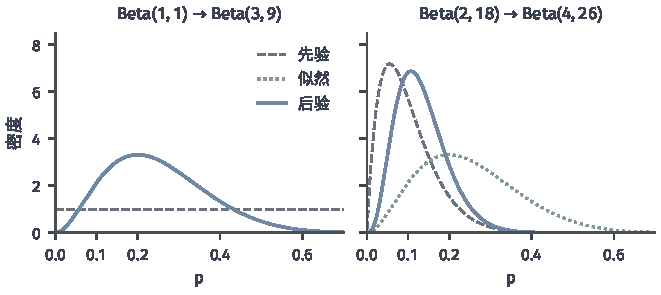
\includegraphics[width=112mm]{figures/01-basic-mathematics/05-probability-and-statistics-basics/matplotlib/est-beta-updating/figure.pdf}
  \caption{抽检数据（$10$件中$2$件不合格）对两种Beta先验的更新。灰色虚线为先验，绿色点线为归一化后的似然$p^2(1-p)^8\times495$，蓝色实线为后验。左：均匀先验$\operatorname{Beta}(1,1)$，后验$\operatorname{Beta}(3,9)$与归一化似然重合。右：先验$\operatorname{Beta}(2,18)$，后验$\operatorname{Beta}(4,26)$介于先验与似然之间。}
  \label{fig:est-beta-updating}
\end{figure}

\paragraph{已知方差的高斯均值模型}
设$\sigma^2$已知，先验$\mu\sim\mathcal{N}(m_0,\tau_0^2)$，观测$x_1,\dots,x_n$在给定$\mu$时独立同分布于$\mathcal{N}(\mu,\sigma^2)$。由例~\ref{ex:est-mle-gaussian-mean}中的平方和分解，似然中依赖$\mu$的部分为$\exp\!\big(-\frac{n(\mu-\bar x)^2}{2\sigma^2}\big)$。乘以先验密度中依赖$\mu$的部分，
\[
\pi(\mu\mid x)\propto\exp\!\Big(-\frac{n(\mu-\bar x)^2}{2\sigma^2}-\frac{(\mu-m_0)^2}{2\tau_0^2}\Big).
\]
为了看出这是什么分布，我们把指数中关于$\mu$的二次式配方。记
\[
\frac{1}{\tau_n^2}=\frac{1}{\tau_0^2}+\frac{n}{\sigma^2},\qquad
m_n=\tau_n^2\Big(\frac{m_0}{\tau_0^2}+\frac{n\bar x}{\sigma^2}\Big).
\]
展开指数中的两个平方，$\mu^2$的系数为$-\frac12\big(\frac{n}{\sigma^2}+\frac1{\tau_0^2}\big)=-\frac{1}{2\tau_n^2}$，$\mu$的系数为$\frac{n\bar x}{\sigma^2}+\frac{m_0}{\tau_0^2}=\frac{m_n}{\tau_n^2}$。因此指数等于$-\frac{\mu^2-2m_n\mu}{2\tau_n^2}$加上一个与$\mu$无关的常数，也就是$-\frac{(\mu-m_n)^2}{2\tau_n^2}$加上常数。常数并入比例因子，得到后验
\begin{equation}
\label{eq:est-gaussian-posterior}
\mu\mid x\ \sim\ \mathcal{N}(m_n,\tau_n^2),\qquad
\frac{1}{\tau_n^2}=\frac{1}{\tau_0^2}+\frac{n}{\sigma^2},\qquad
m_n=\frac{\frac{1}{\tau_0^2}m_0+\frac{n}{\sigma^2}\bar x}{\frac{1}{\tau_0^2}+\frac{n}{\sigma^2}} .
\end{equation}

方差的倒数称为\term{精度}（precision），它度量分布的集中程度。式~\eqref{eq:est-gaussian-posterior}表明两件事。第一，后验精度等于先验精度$1/\tau_0^2$与数据精度$n/\sigma^2$之和，每增加一个观测，精度增加$1/\sigma^2$，所以后验总比先验集中，且随$n$增大越来越集中。第二，后验均值是先验中心$m_0$与样本均值$\bar x$的加权平均，权重与各自的精度成比例：先验越集中，越靠近$m_0$；数据越多或测量越精确，越靠近$\bar x$。

\begin{example}[读数的后验]
\label{ex:est-gaussian-posterior}
取$\sigma=0.2$，先验$\mathcal{N}(10.0,0.1^2)$，数据$n=8$，$\bar x=10.1$。先验精度为$1/0.01=100$，数据精度为$8/0.04=200$，后验精度为$300$，所以$\tau_n^2=1/300$，$\tau_n\approx0.0577$。后验均值
\[
m_n=\frac{100\times10.0+200\times10.1}{300}=\frac{3020}{300}\approx10.067 .
\]
数据的精度是先验的两倍，所以后验均值位于$10.0$与$10.1$之间、离$10.1$更近的三分之二处。
\end{example}

图~\ref{fig:est-gaussian-posterior}画出了这三条曲线。似然曲线以$\bar x=10.1$为中心，标准差为$\sigma/\sqrt n\approx0.071$；先验以$10.0$为中心，标准差为$0.1$；后验中心在两者之间，宽度比两者都窄。

\begin{figure}[htbp]
  \centering
  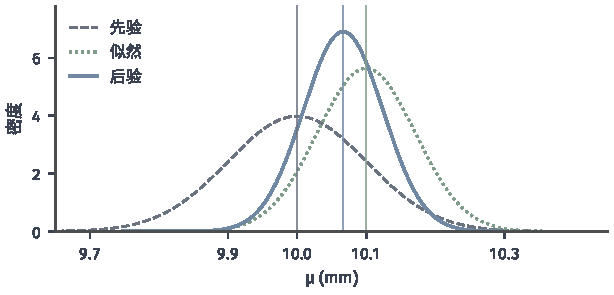
\includegraphics[width=104mm]{figures/01-basic-mathematics/05-probability-and-statistics-basics/matplotlib/est-gaussian-posterior/figure.pdf}
  \caption{已知$\sigma=0.2$时读数均值$\mu$的更新。灰色虚线为先验$\mathcal{N}(10.0,0.1^2)$；绿色点线为归一化的似然，即以$\bar x=10.1$为中心、标准差$0.2/\sqrt8$的高斯曲线；蓝色实线为后验$\mathcal{N}(10.067,1/300)$。三条竖线依次标出$10.0$、$10.067$与$10.1$。}
  \label{fig:est-gaussian-posterior}
\end{figure}

\paragraph{共轭性的含义}
两个例子有一个共同点：先验与后验属于同一个分布族，更新只改变超参数。Beta先验配Bernoulli观测得到Beta后验；高斯先验配已知方差的高斯观测得到高斯后验。

\begin{definition}[共轭先验]
\label{def:est-conjugate-prior}
设$\mathcal{P}$是参数集上的一族分布。若对$\mathcal{P}$中的任一先验和任意观测数据，按式~\eqref{eq:est-bayes}得到的后验仍属于$\mathcal{P}$，则称$\mathcal{P}$是该观测模型的\term{共轭先验}（conjugate prior）族。
\end{definition}

共轭性的计算意义在于：后验不需要数值积分，只需按公式~\eqref{eq:est-beta-posterior}或~\eqref{eq:est-gaussian-posterior}更新几个数。它还使分批处理数据十分方便：先用前一批数据得到后验，再把它当作下一批数据的先验，结果与一次处理全部数据相同。例如抽检数据若分两批，前$5$件含$1$件不合格、后$5$件含$1$件不合格，均匀先验先更新为$\operatorname{Beta}(2,5)$，再更新为$\operatorname{Beta}(3,9)$，与一次更新的结果一致。非共轭的模型中，式~\eqref{eq:est-bayes}的分母通常没有闭式，需要数值方法计算。第~\ref{chap:intervals-tests-prediction}章将用这里的两个后验构造可信区间并预测新观测。

\subsection{后验点估计}

\paragraph{三种常用的点估计}
后验分布完整地描述了看到数据后我们对参数的认识。但很多时候需要报告一个数，例如“不合格率估计为多少”。从后验中提取一个代表值，常用的有三种：
\begin{itemize}
  \item \term{后验均值}（posterior mean）$\mathbb{E}[\theta\mid x]=\int_\Theta\theta\,\pi(\theta\mid x)\,\mathrm{d}\theta$；
  \item \term{后验中位数}（posterior median），即满足$\mathbb{P}(\theta\le a\mid x)=1/2$的$a$；
  \item 后验众数，即后验密度的最大值点，也称\term{最大后验估计}（maximum a posteriori estimate，MAP）。
\end{itemize}
三者分别对应后验分布的“平均位置”“对半分的位置”和“最可能的位置”。前两者可以从另一个角度理解：如果用数$a$去报告$\theta$，并按某种方式衡量报告误差，那么它们分别使不同误差的后验平均最小。

\begin{theorem}[后验均值与后验中位数的最优性]
\label{thm:est-posterior-mean-median}
设后验分布有密度，且$\mathbb{E}[\theta^2\mid x]<\infty$。
\begin{enumerate}
  \item 函数$a\mapsto\mathbb{E}[(\theta-a)^2\mid x]$在$a=\mathbb{E}[\theta\mid x]$处取得唯一最小值。
  \item 记后验分布函数为$G(a)=\mathbb{P}(\theta\le a\mid x)$，并设其密度连续。若$G(a^\ast)=1/2$，则函数$a\mapsto\mathbb{E}[|\theta-a|\mid x]$在$a^\ast$处取得最小值。
\end{enumerate}
\end{theorem}

\begin{proof}
（1）记$\bar\theta=\mathbb{E}[\theta\mid x]$。把$\theta-a$写成$(\theta-\bar\theta)+(\bar\theta-a)$，展开平方并取后验期望，交叉项$2(\bar\theta-a)\mathbb{E}[\theta-\bar\theta\mid x]=0$，于是
\[
\mathbb{E}[(\theta-a)^2\mid x]=\operatorname{Var}(\theta\mid x)+(\bar\theta-a)^2 .
\]
第一项不依赖$a$，第二项在$a=\bar\theta$时为零、其余时候为正。

（2）记后验密度为$g$，则
\[
h(a)=\mathbb{E}[|\theta-a|\mid x]=\int_{-\infty}^a(a-\theta)g(\theta)\,\mathrm{d}\theta+\int_a^{\infty}(\theta-a)g(\theta)\,\mathrm{d}\theta .
\]
按积分上下限求导（第~\ref{chap:univariate-integration}章），两个积分的边界项在$\theta=a$处都为零，得
\[
h'(a)=\int_{-\infty}^a g(\theta)\,\mathrm{d}\theta-\int_a^{\infty}g(\theta)\,\mathrm{d}\theta=2G(a)-1 .
\]
$G$不减，所以$h'(a)$在$a<a^\ast$时不大于$0$，在$a>a^\ast$时不小于$0$；$h$在$a^\ast$左侧不增、右侧不减，故在$a^\ast$处取得最小值。
\end{proof}

因此，若报告误差按平方计，应报告后验均值；若按绝对值计，应报告后验中位数。后验众数没有类似的平方或绝对误差解释，它的含义是“后验密度最高的位置”。当先验是均匀分布时，后验密度与似然成比例，后验众数就是最大似然估计。

\paragraph{Beta后验的点估计}
对后验$\operatorname{Beta}(a',b')$，其中$a'=a+k$，$b'=b+n-k$，后验均值为$\frac{a'}{a'+b'}$。后验众数需要分情况：$a',b'>1$时密度在内部有唯一最大值点$\frac{a'-1}{a'+b'-2}$；$a'\le1$或$b'\le1$时，密度在内部没有极大值点：例如$a'=1<b'$时，密度$b'(1-p)^{b'-1}$在端点$p=0$处最大；$a'<1$时，密度在$p\to0$时无界，众数不存在；$a'=b'=1$时密度为常数，每一点都是众数。后验中位数没有初等闭式，需要数值计算。

\begin{example}[抽检数据的三种后验估计]
\label{ex:est-beta-point-estimates}
在均匀先验下，后验为$\operatorname{Beta}(3,9)$：后验均值为$3/12=0.25$，后验众数为$2/10=0.2$，数值计算得后验中位数约为$0.236$。众数等于最大似然估计$0.2$，这正是均匀先验下两者一致的体现。图~\ref{fig:est-posterior-summaries}显示，这个后验向右偏斜，右侧的长尾把均值拉到中位数右侧，众数则在三者中最小。

在先验$\operatorname{Beta}(2,18)$下，后验为$\operatorname{Beta}(4,26)$，均值约为$0.133$，众数为$3/28\approx0.107$，中位数约为$0.125$，三者都小于样本比例$0.2$，反映了先验的影响。

若$10$件全部合格，均匀先验下的后验为$\operatorname{Beta}(1,11)$，其密度$11(1-p)^{10}$在$p=0$处最大，所以后验众数为$0$，与最大似然估计相同；但后验均值为$1/12\approx0.083$，后验中位数为$1-2^{-1/11}\approx0.061$，二者都在$(0,1)$内部。与例~\ref{ex:est-mle-boundary}中的$\hat p=0$相比，它们避免了“永不出次品”的结论。
\end{example}

\begin{figure}[htbp]
  \centering
  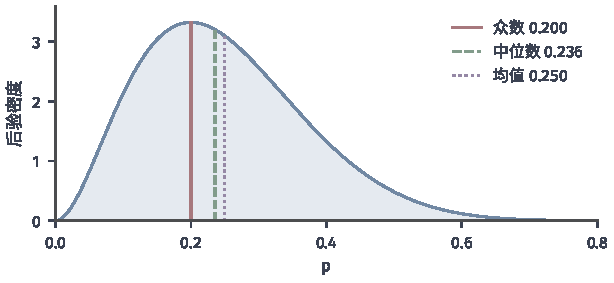
\includegraphics[width=104mm]{figures/01-basic-mathematics/05-probability-and-statistics-basics/matplotlib/est-posterior-summaries/figure.pdf}
  \caption{偏斜的后验$\operatorname{Beta}(3,9)$上三种点估计的位置。红色实线为后验众数$0.2$，绿色虚线为后验中位数约$0.236$，紫色点线为后验均值$0.25$。分布的右尾较长，使均值位于中位数右侧。}
  \label{fig:est-posterior-summaries}
\end{figure}

\paragraph{对称后验与存在性}
对高斯后验$\mathcal{N}(m_n,\tau_n^2)$，密度关于$m_n$对称且在$m_n$处唯一取得最大值，所以后验均值、中位数和众数都等于$m_n$。对读数数据，三者都约为$10.067$。

一般情况下，三种点估计的存在性和唯一性都不能一概假定。后验均值要求后验期望存在；中位数可能在一个区间上都满足$G(a)=1/2$，此时不唯一；众数可能不唯一，也可能不存在。例如后验$\operatorname{Beta}(0.5,0.5)$的密度在$p\to0$和$p\to1$时都趋于无穷，没有最大值点，而它的均值和中位数都是$0.5$，恰好位于密度最低的地方。报告后验点估计时，最好同时查看后验分布的形状。

\section{本章小结}
\label{sec:est-summary}

本章从“由有限数据了解总体规律”这一问题出发，建立了一条对象链：总体规律由统计模型$\{F_\theta:\theta\in\Theta\}$表示；随机样本$X_1,\dots,X_n$是独立同分布的随机变量，其联合分布由式~\eqref{eq:est-sample-joint}的乘积给出；统计量是不含未知参数的样本函数，用于估计时称为估计量，代入数据后得到估计值。独立同分布是对抽样方式的假设，不放回抽样和时间序列等情形需要另行检查。

在不假定模型时，经验分布把概率$1/n$放在每个观测上，经验分布函数、样本矩、样本方差和样本分位数都是它的数值特征。修正样本方差的分母$n-1$来自平方离差和的期望$(n-1)\sigma^2$；样本分位数在跳跃处有多种约定，小样本时需要说明所用的约定。

三类估计使用了不同的信息。矩估计只使用几个样本矩，计算简单，但要检查矩是否存在、能否确定参数、解是否落在参数集中并与数据相容。最大似然估计使用模型的整个联合分布，在常见模型中化为求导和配方，但令导数为零不能代替对边界解和无界似然的检查。基于后验的估计额外使用先验信息，Bayes公式把先验与似然合并为后验；在Beta--Bernoulli和已知方差的高斯均值这两个共轭模型中，后验均值都是先验中心与样本均值的加权平均，权重由先验的等效样本量或精度决定。从后验中提取均值、中位数和众数，分别对应平方误差、绝对误差和密度最高这三种标准。

用全章的两组数据比较：不合格率的矩估计和最大似然估计都是$0.2$，均匀先验下后验均值为$0.25$、后验众数为$0.2$；读数均值的三种估计依次为$10.1$、$10.1$与$10.067$，方差的矩估计和最大似然估计都是$0.035$，修正样本方差为$0.04$。同一个参数有多个估计，它们在当前数据上给出不同的数，单凭一组数据无法判断哪一个更接近真值。要比较它们，就要回到抽样之前，研究估计量作为随机变量的分布：它的中心在哪里，波动有多大，样本量增加时如何变化。这正是第~\ref{chap:sampling-errors}章的内容。
